\documentclass[tikz,crop,convert={density=300,outext=.png},border=0.0cm,width=18cm,height=7cm]{standalone}
%\documentclass[tikz,border=0.3cm]{standalone}
%\usepackage[left=2.2cm,right=2.2cm,top=2.5cm,bottom=2.0cm,a4paper]{geometry}
\usepackage{pgfplots}
\usepackage{amsmath}
\usepackage{physics}

\definecolor{one}{RGB}{0,68,27}
\definecolor{two}{RGB}{35,139,69}
\definecolor{three}{RGB}{153,216,201}
\pgfplotsset{compat=newest,
    %width=6cm,
    %height=3cm,
    scale only axis=true,
    max space between ticks=25pt,
    try min ticks=5,
    every axis/.style={
        axis y line=middle,
        axis x line=middle,
        axis line style={thick,->,>=latex, shorten >=-.3cm}
    },
      every axis plot/.append style={thick},
    tick style={black, thick},
}
\tikzset{
    semithick/.style={line width=0.8pt},
  }
\usetikzlibrary{shapes.geometric, arrows}  
\usepgfplotslibrary{groupplots}
\usepgfplotslibrary{dateplot}
\usetikzlibrary{positioning}
%\pgfplotsset{compat=1.17}

\begin{document}
\begin{tikzpicture}
% Row 1 out of 2
\node[inner sep=0pt] (mixed) at (-6,1.67)
{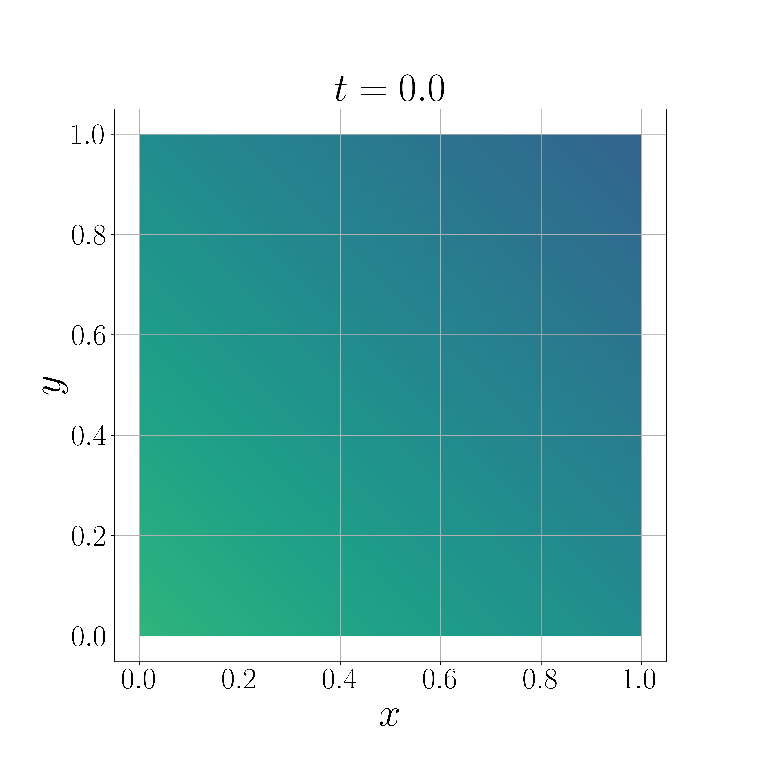
\includegraphics[width=3.6cm,page=1]{{./individual_figures_PDE}}};
\node[inner sep=0pt] (mixed) at (-3,1.67)
{\includegraphics[width=3.6cm,page=2]{{./individual_figures_PDE}}};
\node[inner sep=0pt] (mixed) at (0,1.67)
{\includegraphics[width=3.6cm,page=3]{{./individual_figures_PDE}}};
\node[inner sep=0pt] (mixed) at (3,1.67)
{\includegraphics[width=3.6cm,page=4]{{./individual_figures_PDE}}};
\node[inner sep=0pt] (mixed) at (6,1.67)
{\includegraphics[width=3.6cm,page=5]{{./individual_figures_PDE}}};
% Row 2 out of 2
\node[inner sep=0pt] (mixed) at (-6,-1.67)
{\includegraphics[width=3.6cm,page=6]{{./individual_figures_PDE}}};
\node[inner sep=0pt] (mixed) at (-3,-1.67)
{\includegraphics[width=3.6cm,page=7]{{./individual_figures_PDE}}};
\node[inner sep=0pt] (mixed) at (0,-1.67)
{\includegraphics[width=3.6cm,page=8]{{./individual_figures_PDE}}};
\node[inner sep=0pt] (mixed) at (3,-1.67)
{\includegraphics[width=3.6cm,page=9]{{./individual_figures_PDE}}};
\node[inner sep=0pt] (mixed) at (6,-1.67)
{\includegraphics[width=3.6cm,page=10]{{./individual_figures_PDE}}};

% % Lines
% \draw (-7.6,-3.5) -- (-7.6,3.5);
% \draw (-7.7,3.17) -- (7.7,3.17);
% \draw (-7.6,-0.17) -- (7.6,-0.17);
% \draw (-7.7,-3.17) -- (7.7,-3.17);
% Labels of all sub figures
\node (a) at (-7.85,3.17) {\small (\textbf{A})};
\node (a) at (-7.85,-0.17) {\small (\textbf{B})};
% \node[right=4.15cm of a] (b) {(\textbf{B})};
%\node[right=4.20cm of b] (c) {(\textbf{C})};


\node[inner sep=0pt] (mixed) at (7.85,0)
{
\includegraphics[scale=0.265]{{./colourbar}}};
\node (a) at (8.55,3.1) {$u_{\max}$};
\node[rotate=270] (a) at (8.5,0) {$u(x,y,t)$};
\node (a) at (8.55,-3.1) {$u_{\min}$};

% Horizontal line
\draw [->,thin,line width=1mm,-latex] (-7.5,-3.75) -- (7.5,-3.75);
\node at (0,-4.25) {\small\textit{Increasing time,} $t$};

\end{tikzpicture}

\end{document}

